\chapter{Resultados y discusión}
\label{ch:resultados}

Este capítulo presenta y analiza los resultados del experimento descrito en
el Capítulo~\ref{ch:metodologia}. Se evalúan 6 carteras optimizadas (tres
clásicas, una por estimador de $\boldsymbol{\Sigma}$, y tres con
$\boldsymbol{\mu}$ predicho por ML) y 2 baselines pasivos sobre 143 meses
out-of-sample (enero 2013 -- diciembre 2024).

%--------------------------------------------------------------------
\section{Comparación global de carteras}
%--------------------------------------------------------------------

La Tabla~\ref{tab:resultados-globales} presenta las métricas de todas las
carteras evaluadas. La Figura~\ref{fig:sharpe-comparacion} ordena las
estrategias por ratio de Sharpe y la Figura~\ref{fig:valor-acumulado}
muestra la evolución del valor acumulado de 1\texteuro{} invertido.

\begin{table}[htbp]
    \centering
    \caption{Resultados completos del backtesting walk-forward
             (enero 2013 -- diciembre 2024, 143 meses).}
    \label{tab:resultados-globales}
    \resizebox{\textwidth}{!}{\begin{tabular}{lrrrrrrr}
\toprule
Estrategia & Rent. anual (\%) & Vol. anual (\%) & Sharpe & Máx. DD (\%) & Turnover & HHI & Nº activos \\
\midrule
Markowitz (muestral) & 8,34 & 12,97 & 0,64 & 32,26 & 0,14 & 0,15 & 8,85 \\
Markowitz (Ledoit-Wolf) & 8,86 & 12,99 & 0,68 & 29,30 & 0,13 & 0,14 & 10,62 \\
Markowitz (PCA) & 9,00 & 13,01 & 0,69 & 30,91 & 0,14 & 0,16 & 8,57 \\
Markowitz + Ridge & 9,29 & 13,72 & 0,68 & 18,42 & 0,57 & 0,14 & 11,17 \\
Markowitz + Lasso & 9,65 & 12,79 & 0,75 & 25,55 & 0,12 & 0,10 & 14,89 \\
Markowitz + RF & 9,84 & 13,91 & 0,71 & 24,09 & 0,36 & 0,12 & 13,62 \\
1/N (equiponderada) & 10,68 & 14,14 & 0,76 & 21,89 & 0,00 & 0,03 & 30,00 \\
SPY (mercado) & 12,94 & 14,42 & 0,90 & 25,48 & 0,00 & 1,00 & 1,00 \\
\bottomrule
\end{tabular}
}
\end{table}

\begin{figure}[htbp]
    \centering
    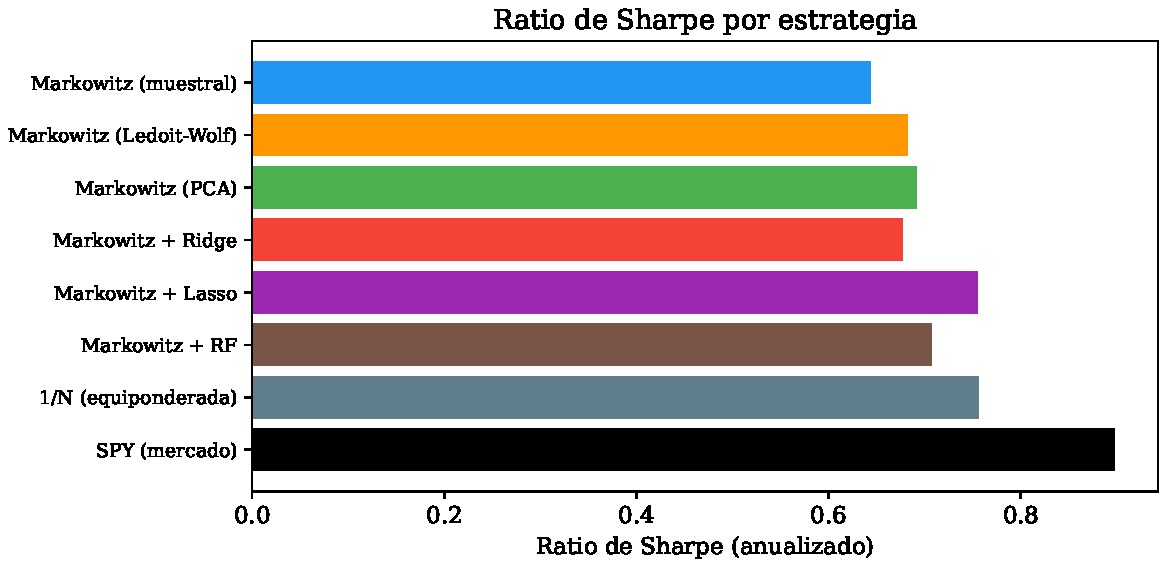
\includegraphics[width=0.56\textwidth]{../data/outputs/sharpe_comparacion}
    \caption{Ratio de Sharpe anualizado por estrategia.}
    \label{fig:sharpe-comparacion}
\end{figure}

\begin{figure}[htbp]
    \centering
    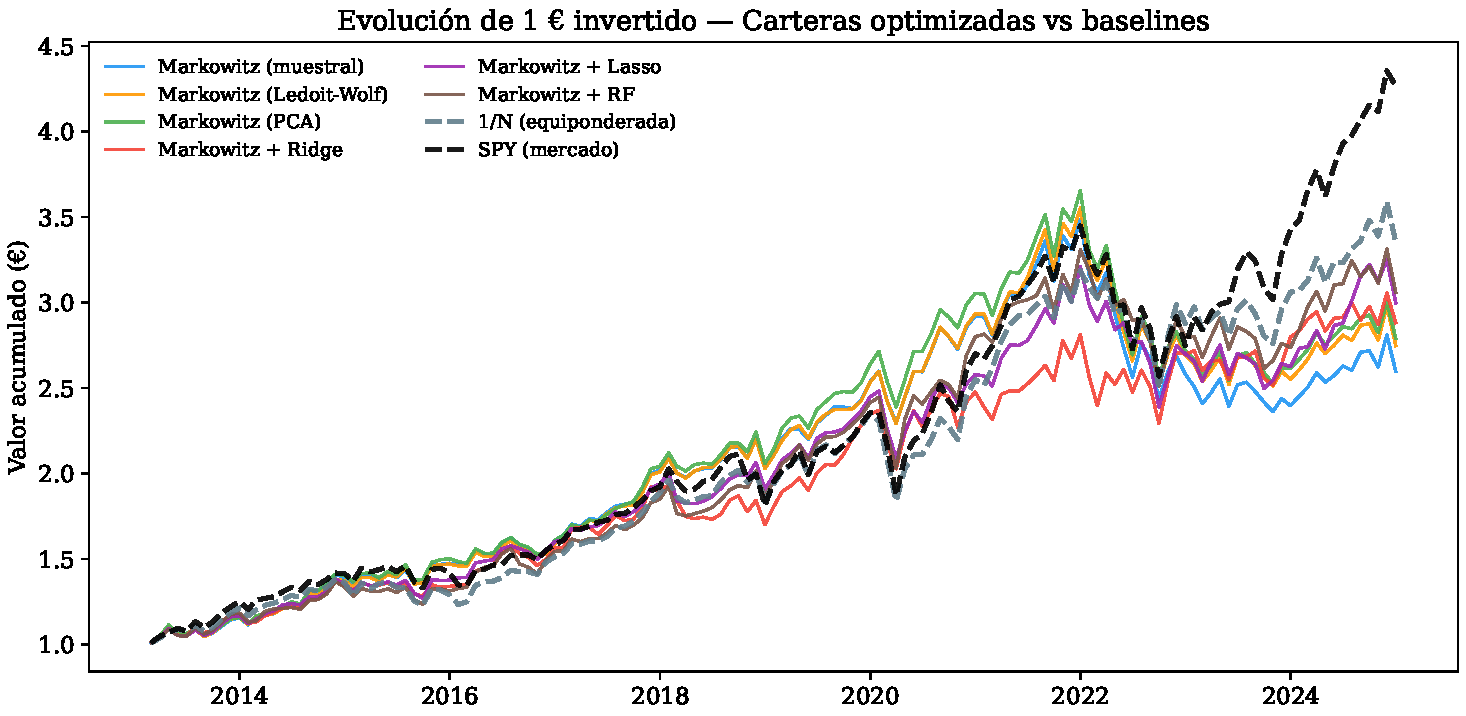
\includegraphics[width=0.66\textwidth]{../data/outputs/valor_acumulado}
    \caption{Evolución de 1\texteuro{} invertido en cada estrategia
             durante el periodo out-of-sample (2013--2024). Las líneas
             discontinuas representan los baselines pasivos.}
    \label{fig:valor-acumulado}
\end{figure}

\subsection{Resultado principal}

El hallazgo más relevante es que \textbf{ninguna cartera optimizada supera
a los baselines pasivos} en ratio de Sharpe. El SPY obtiene un Sharpe de
$0{,}90$ con una rentabilidad anualizada del $12{,}9\%$, y la cartera
$1/N$ equiponderada alcanza un Sharpe de $0{,}76$ con un $10{,}7\%$
anualizado.

Entre las carteras optimizadas, la \textbf{Markowitz + Lasso} es la mejor,
con un Sharpe de $0{,}75$ y una rentabilidad del $9{,}7\%$ anualizado, hasta
el punto de \emph{igualar} en la práctica a la cartera $1/N$ ($0{,}76$).
Le siguen \textbf{Markowitz + RF} (Sharpe $0{,}71$) y \textbf{Markowitz (PCA)}
($0{,}69$). No obstante, como se demuestra en la
Sección~\ref{sec:significancia}, ninguna de estas diferencias es
estadísticamente significativa.

Este resultado es consistente con la literatura: DeMiguel, Garlappi y Uppal
\cite{DeMiguel2009} demostraron que se necesitan ventanas de estimación
extremadamente largas (más de 3.000 meses) para que las carteras optimizadas
superen consistentemente a la $1/N$. Con 36 meses de ventana, el error de
estimación domina cualquier ganancia teórica de la optimización.

\subsection{Rentabilidad frente a riesgo}

Todas las carteras optimizadas presentan volatilidades muy similares
(12,8\%--13,9\% anual), cercanas a las de los baselines (14,1\%--14,4\%).
La diferencia está en la rentabilidad: el SPY genera un $12{,}9\%$ frente
al $8{,}3\%$--$9{,}8\%$ de las carteras optimizadas. Esto sugiere que el
principal lastre de las carteras optimizadas no es un exceso de riesgo,
sino una \textbf{rentabilidad sistemáticamente menor}: los activos que
selecciona el optimizador rinden, fuera de muestra, menos que el mercado.

%--------------------------------------------------------------------
\section{Efecto del estimador de covarianza}
%--------------------------------------------------------------------

La Tabla~\ref{tab:resultados-globales} permite comparar el efecto de los
tres estimadores de $\boldsymbol{\Sigma}$ cuando $\boldsymbol{\mu}$ se
estima como media histórica.

El estimador \textbf{muestral} es el peor (Sharpe $0{,}64$), con la mayor
concentración (HHI $0{,}15$; $8{,}9$ activos). \textbf{Ledoit-Wolf} lo mejora en
$+0{,}04$ ($0{,}68$), reduce la concentración (HHI $0{,}14$; $10{,}6$ activos) y
baja el drawdown ($29{,}3\%$ frente a $32{,}3\%$). \textbf{PCA} logra el mejor
Sharpe clásico ($0{,}69$), algo más rentable pero más concentrado (HHI $0{,}16$;
$8{,}6$ activos).

Esto confirma el análisis del Capítulo~\ref{ch:limitaciones}: Ledoit-Wolf da
las carteras más diversificadas y estables y el estimador muestral es el más
vulnerable al error de estimación, con PCA en una posición intermedia ---mejor
rentabilidad, pero menor diversificación.

%--------------------------------------------------------------------
\section{Efecto de la predicción ML de \texorpdfstring{$\boldsymbol{\mu}$}{μ}}
%--------------------------------------------------------------------

\subsection{Rendimiento de las carteras ML}

Las tres estrategias ML utilizan el estimador de covarianza Ledoit-Wolf y
se diferencian únicamente en el modelo de predicción de $\boldsymbol{\mu}$:

\begin{itemize}
    \item \textbf{Lasso} (Sharpe $0{,}75$) es la \textbf{mejor cartera
          optimizada} y prácticamente iguala a la $1/N$, con el menor turnover
          ($0{,}12$) y la mayor diversificación de las carteras optimizadas
          (14,9 activos, HHI $0{,}10$).
    \item \textbf{Random Forest} ($0{,}71$), el único modelo no lineal, queda
          en segundo lugar, con un turnover moderado ($0{,}36$).
    \item \textbf{Ridge} ($0{,}68$) se queda en el Sharpe del clásico de
          Ledoit-Wolf, pero logra el \textbf{menor drawdown del estudio}
          ($18{,}4\%$).
\end{itemize}

\subsection{Análisis del rendimiento de los modelos ML}

El factor decisivo es el \textbf{tamaño efectivo de la muestra de
entrenamiento}. Al estimar un único modelo agrupado sobre todos los activos
(Capítulo~\ref{ch:ml}), cada ajuste dispone de unas $30 \times 36 \approx 1.000$
observaciones en lugar de 36. Por eso incluso Random Forest se comporta de forma
estable (Sharpe $0{,}71$): con solo 36 observaciones por activo un modelo no
lineal sobreajustaría el ruido, pero con la muestra agrupada extrae una señal
débil pero consistente.

Entre los lineales, Lasso supera a Ridge: la regularización $\ell_1$ anula los
coeficientes sin poder predictivo (selección automática) y, en un entorno de muy
baja señal-ruido, produce predicciones parsimoniosas y estables ---de ahí el
bajísimo turnover de Lasso. De hecho, en muchos meses la validación cruzada elige
un nivel que anula todos los coeficientes y reduce $\hat{\boldsymbol{\mu}}$ a una
constante: cuando los datos no contienen señal aprovechable, el modelo lo
refleja tal cual, en lugar de forzar una predicción ruidosa. Todo ello es coherente con la literatura \cite{Gu2020}, que
subraya compartir información entre activos y regularizar con fuerza cuando los
datos escasean.

\subsection{Turnover y costes de transacción}

La Tabla~\ref{tab:resultados-globales} muestra que el turnover varía
notablemente: las estrategias con $\boldsymbol{\mu}$ histórico tienen un
turnover de $0{,}13$--$0{,}14$, frente al $0{,}12$ de Lasso, el $0{,}36$ de RF
y el $0{,}57$ de Ridge.

Frente al resultado habitual de que el ML dispara el turnover,
aquí el modelo más parsimonioso (Lasso) alcanza uno incluso
\emph{inferior} al de las estrategias clásicas, mientras que Ridge ---que
mantiene activas todas las features--- es el que más rota. Aun así, los costes
de transacción siguen siendo relevantes para Ridge y RF: con un coste del
$0{,}1\%$ por operación, el impacto anual aproximado ($12 \times
\text{turnover} \times 0{,}001$) restaría en torno a $0{,}4$--$0{,}7$ puntos
porcentuales de rentabilidad a esas dos estrategias, frente a apenas $0{,}1$
en el caso de Lasso.

El matiz práctico es importante: \textbf{el coste de transacción no penaliza
al ML en bloque, sino a los modelos cuyas predicciones de $\boldsymbol{\mu}$
son inestables mes a mes}.

%--------------------------------------------------------------------
\section{Estabilidad temporal}
%--------------------------------------------------------------------

La Figura~\ref{fig:valor-acumulado} muestra que todas las estrategias
optimizadas siguen trayectorias similares hasta aproximadamente 2018, cuando el
SPY se despega,
impulsado por el excepcional mercado estadounidense de 2019--2024 (recuperación
post-COVID, auge de las grandes tecnológicas). Es notable que la $1/N$, con cero
turnover y máxima diversificación, siga de cerca al SPY hasta 2020: refuerza que
la diversificación ingenua es difícil de batir, sobre todo en mercados
concentrados donde unas pocas acciones (Apple, Microsoft, NVIDIA) generan la
mayor parte de la rentabilidad del índice.

%--------------------------------------------------------------------
\section{Significancia estadística}
\label{sec:significancia}
%--------------------------------------------------------------------

Comparar ratios de Sharpe con una única muestra de 143 meses sin medir su
incertidumbre puede ser engañoso: una diferencia de centésimas puede deberse al
ruido muestral. Para cuantificarlo se emplean dos herramientas complementarias
(Tabla~\ref{tab:significancia}): un \textbf{intervalo de confianza al 95\,\%} del
Sharpe por \textit{bootstrap} de bloques ---que preserva la autocorrelación--- y
el \textbf{test de Jobson-Korkie con la corrección de Memmel} \cite{Memmel2003},
que contrasta si dos estrategias tienen el mismo Sharpe frente a cada baseline
(SPY y $1/N$).

\begin{table}[htbp]
    \centering
    \caption{Significancia estadística de los ratios de Sharpe: intervalo de
             confianza al 95\,\% por \textit{bootstrap} y $p$-valor del test de
             Memmel frente a cada baseline. El Sharpe de esta tabla se calcula
             como media/desviación típica mensual anualizada, ligeramente
             superior al de la Tabla~\ref{tab:resultados-globales} (geométrico)
             por el efecto del \textit{volatility drag}.}
    \label{tab:significancia}
    \small
    \begin{tabular}{lrrrrr}
\toprule
Estrategia & Sharpe & IC 95\% inf. & IC 95\% sup. & $p$ vs SPY & $p$ vs 1/N \\
\midrule
Markowitz (muestral) & 0,685 & 0,205 & 1,245 & 0,207 & 0,554 \\
Markowitz (Ledoit-Wolf) & 0,720 & 0,249 & 1,274 & 0,259 & 0,680 \\
Markowitz (PCA) & 0,729 & 0,249 & 1,298 & 0,292 & 0,727 \\
Markowitz + Ridge & 0,718 & 0,260 & 1,235 & 0,263 & 0,642 \\
Markowitz + Lasso & 0,787 & 0,302 & 1,367 & 0,477 & 0,977 \\
Markowitz + RF & 0,746 & 0,282 & 1,277 & 0,334 & 0,752 \\
1/N (equiponderada) & 0,792 & 0,305 & 1,358 & 0,206 & --- \\
SPY (mercado) & 0,921 & 0,399 & 1,559 & --- & 0,206 \\
\bottomrule
\end{tabular}

\end{table}

Los resultados son contundentes: \textbf{ninguna diferencia de Sharpe es
estadísticamente significativa}. Todos los $p$-valores superan el 5\,\% ---
ninguno baja de $0{,}20$---, e incluso comparar los dos baselines (SPY frente a
$1/N$) da $p = 0{,}21$; los intervalos de confianza son además muy anchos (p.\
ej.\ $[0{,}40,\ 1{,}56]$ para el SPY, $[0{,}30,\ 1{,}37]$ para Lasso) y se
solapan por completo. La lectura refuerza la tesis del trabajo: con 143 meses,
\textbf{el error de estimación del propio Sharpe es tan grande que no permite
afirmar que ninguna estrategia ---ni siquiera el mercado--- sea superior a las
demás}. Las diferencias de la Tabla~\ref{tab:resultados-globales}, aunque
económicamente sugerentes, deben leerse con esta cautela.

%--------------------------------------------------------------------
\section{Discusión crítica}
%--------------------------------------------------------------------

\subsection{¿Por qué no se baten los baselines pasivos?}

Los resultados muestran que, aunque la mejor estrategia con ML (Lasso) llega a
igualar a la cartera $1/N$, ninguna estrategia ---optimizada o pasiva--- se
distingue estadísticamente del resto, y todas quedan por debajo del SPY en
términos puntuales. Varias razones lo explican:

\begin{enumerate}
    \item \textbf{Señal débil:} la predictibilidad de las rentabilidades
          mensuales a partir de información de precio es muy limitada ---los
          $R^2$ de la literatura de \textit{return prediction} rara vez superan
          el $2\%$ \cite{Gu2020}. El enfoque agrupado eleva el tamaño efectivo
          de entrenamiento a unas 1.000 observaciones y estabiliza los modelos,
          pero más datos no crean una señal inexistente: la regularización
          óptima descarta a menudo toda la señal.
    \item \textbf{Inestabilidad de las predicciones:} en los modelos cuyas
          predicciones rotan mucho (Ridge y, menos, RF), los cambios en
          $\hat{\boldsymbol{\mu}}$ elevan el turnover y los costes implícitos.
    \item \textbf{El QP amplifica el error:} el optimizador es muy sensible a
          los errores en $\boldsymbol{\mu}$ \cite{Merton1980}; una pequeña
          sobrestimación puede dar a un activo un peso desproporcionado.
\end{enumerate}

\subsection{Limitaciones del estudio}

\begin{itemize}
    \item \textbf{Sesgo de supervivencia:} solo constituyentes actuales del
          S\&P 500, lo que sobrestima algo las rentabilidades del universo.
    \item \textbf{Sin costes de transacción explícitos:} el turnover se
          reporta pero no se descuenta, lo que favorece a las estrategias que
          más rotan.
    \item \textbf{Ventana única:} el periodo 2013--2024 fue excepcionalmente
          alcista en EE.UU.; los resultados podrían diferir en otros mercados.
    \item \textbf{Features y modelos limitados:} solo features de precio y tres
          modelos; variables fundamentales o arquitecturas más sofisticadas
          (gradient boosting, redes) podrían ayudar, a costa de más datos.
\end{itemize}

\subsection{Implicaciones}

Que ninguna estrategia optimizada se distinga estadísticamente de los baselines
pasivos no debe leerse como un fracaso del enfoque, sino como una validación
empírica de la dificultad fundamental de seleccionar carteras con parámetros
estimados ---la misma dificultad que justifica seguir investigando en
estimadores robustos y métodos de predicción. Que Lasso sea la mejor cartera
optimizada e iguale a la $1/N$ ---con bajo turnover y alta diversificación---
sugiere que combinar un buen estimador de covarianza (Ledoit-Wolf) con una
predicción regularizada y parsimoniosa es una dirección razonable; pero, a falta
de significancia estadística, esa mejora no puede darse por establecida con los
datos disponibles, y confirmarla exigiría horizontes más largos, más activos o
features adicionales.
